\documentclass{article}
\usepackage[british]{babel}
\usepackage{../lib/tex/naproche}
\documentclass[12pt,oneside]{book}

\usepackage[foundations]{../../lib/tex/naproche}
\usepackage{../../lib/tex/libraries}
\usepackage{graphicx}
\usepackage{float}
\usepackage{caption}
\usepackage{footnote}

\makesavenoteenv{tabular} % Make footnotes work in tabular environments


\title{Foundations of Mathematics}
\author{Marcel Schütz}
\date{2022}

\begin{document}
  \maketitle

  \tableofcontents

  \begin{figure}[H]
    \centering
    \fbox{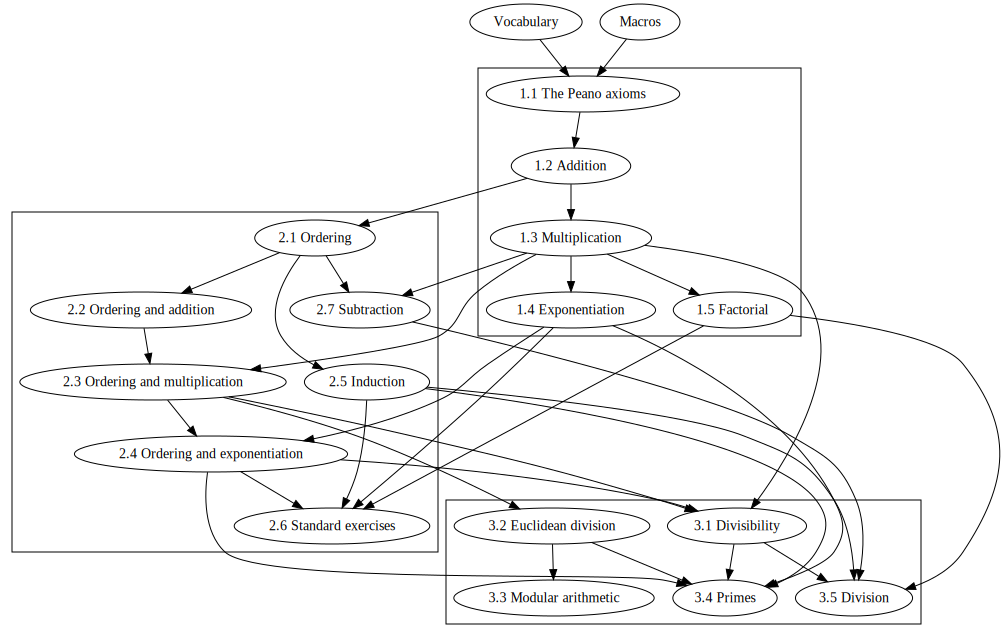
\includegraphics[width=0.9\linewidth]{./dependency-graph/graph.png}}
    \caption*{Interdependencies of the chapters}
  \end{figure}


  \section*{Introduction}

  This is a library providing a foundation of mathematics based on a
  Kelley-Morse like class theory with urelements.
  It introduces common operations on classes like unions or intersections
  (\cref{chapter:classes}) together with detailed proofs of their algebraic
  properties (\cref{chapter:computation-laws-for-classes}), the symmetric
  difference of two classes (\cref{chapter:symmetric-difference}) and the
  notions of ordered pairs and Cartesian products
  (\cref{chapter:pairs-and-products}) as well as proofs of the algebraic
  properties of the latter (\cref{chapter:computation-laws-for-products}).
  Moreover, it provides common operations on maps (\cref{chapter:maps}), various
  properties of images and preimages (\cref{chapter:image-and-preimage}) and the
  notions of injectivity, surjectivity, bijectivity
  (\cref{chapter:injections-surjections-bijections}) and invertibility of maps
  (\cref{chapter:invertible-maps}).
  The library provides an axiom system characterizing sets (\cref{chapter:sets})
  and, furthermore, it covers the notions of binary relations
  (\cref{chapter:binary-relations}), fixed-points of subset preserving maps
  (\cref{chapter:fixed-points}), including and equinumerosity
  (\cref{chapter:equinumerosity}).

  As two famous results it includes the Knaster-Tarski fixed point theorem
  (\cref{FOUNDATIONS_12_8420450166112256}) and the Cantor-Schröder-Bernstein
  theorem (\cref{FOUNDATIONS_13_1913663275401216}).

  \paragraph*{Usage.}
  At the very beginning of each chapter you can find the name of its source
  file, e.g. \path{foundations/sections/01_classes.ftl.tex} for
  \cref{chapter:classes}. This filename can be used to import the chapter via
  \Naproche's \texttt{readtex} instruction to another ForTheL text, e.g.:
  \begin{center}
    \verb`[readtex \path{foundations/sections/01_classes.ftl.tex}]`
  \end{center}

  \paragraph*{Checking times.}
  The checking times for each of the chapters may vary from computer to
  computer, but on mid-range hardware they are likely to be similar to those
  given in table below:

  \begin{center}
    \begin{tabular}{c|c|c}

      & \multicolumn{2}{c}{\textbf{Checking time}}
      \\
      \textbf{Chapter}
      & \textbf{without dependencies}     & \textbf{with dependencies}
      \\ \hline
      \ref{chapter:classes}
      & 00:04 min                         & 00:04 min
      \\
      \ref{chapter:computation-laws-for-classes}
      & 00:12 min                         & 00:16 min
      \\
      \ref{chapter:symmetric-difference}
      & 00:32 min                         & 00:48 min
      \\
      \ref{chapter:pairs-and-products}
      & 00:08 min                         & 00:12 min
      \\
      \ref{chapter:computation-laws-for-products}
      & 01:36 min                         & 01:56 min
      \\
      \ref{chapter:maps}
      & 01:13 min                         & 01:25 min
      \\
      \ref{chapter:image-and-preimage}
      & 01:28 min                         & 02:53 min
      \\
      \ref{chapter:injections-surjections-bijections}
      & 00:38 min                         & 02:03 min
      \\
      \ref{chapter:invertible-maps}
      & 02:20 min                         & 04:23 min
      \\
      \ref{chapter:sets}
      & 02:17 min                         & 06:40 min
      \\
      \ref{chapter:binary-relations}
      & 00:14 min                         & 06:54 min
      \\
      \ref{chapter:fixed-points}
      & 00:33 min                         & 07:13 min
      \\
      \ref{chapter:equinumerosity}
      & 01:48 min                         & 09:01 min
    \end{tabular}
  \end{center}


  \subfile{sections/01_classes.ftl.tex}
  \subfile{sections/02_computation-laws-for-classes.ftl.tex}
  \subfile{sections/03_symmetric-difference.ftl.tex}
  \subfile{sections/04_pairs-and-products.ftl.tex}
  \subfile{sections/05_computation-laws-for-products.ftl.tex}
  \subfile{sections/06_maps.ftl.tex}
  \subfile{sections/07_image-and-preimage.ftl.tex}
  \subfile{sections/08_injections-surjections-bijections.ftl.tex}
  \subfile{sections/09_invertible-maps.ftl.tex}
  \subfile{sections/10_sets.ftl.tex}
  \subfile{sections/11_binary-relations.ftl.tex}
  \subfile{sections/12_fixed-points.ftl.tex}
  \subfile{sections/13_equinumerosity.ftl.tex}
\end{document}

\usepackage{amssymb}

\newcommand{\Nat}{\mathbb{N}}
\newcommand{\Prime}{\mathbb{P}}
\renewcommand{\succ}{\textrm{succ}}
\newcommand{\pred}{\textrm{pred}}
\newcommand{\add}{\textrm{add}}
\newcommand{\mul}{\textrm{mul}}
\renewcommand{\exp}{\textrm{exp}}
\newcommand{\fac}{\textrm{fac}}
\renewcommand{\div}{\mathop{\textrm{div}}}
\renewcommand{\mod}{\mathop{\textrm{mod}}}


\title{Dedekind's Recursion Theorem}
\author{\Naproche formalization: \vspace{0.5em} \\
Marcel Schütz}
\date{2024}

\begin{document}
  \maketitle

  \noindent This is a formalization of Dedekind's recursion theorem.
  It states that for any function $f : A \to A$ and any $a \in A$
  there exists a unique function
  $\varphi : \Nat \to A$ that is \emph{recursively defined} by
  $f$ and $a$, i.e. $\varphi(0) = a$ and
  $\varphi(n + 1) = f(\varphi(n))$.
  (cf. \cite{Ebbinghaus1991}).

  \begin{imports}
    \begin{forthel}
      [prove off][check off]
      [readtex \path{libraries/source/arithmetics/01_natural-numbers.ftl.tex}]
      [prove on][check on]
      Let $n + 1$ stand for $\succ(n)$.
    \end{forthel}
  \end{imports}

  \begin{forthel}
    \begin{definition*}\label{ARITHMETIC_02_4608408013504512}
      Let $a$ be an object and $f$ be a map.
      Let $\varphi$ be a map from $\Nat$ to $\dom(f)$.
      $\varphi$ is recursively defined by $a$ and $f$ iff $\varphi(0) = a$ and $\varphi(n + 1) = f(\varphi(n))$ for every $n \in \Nat$.
    \end{definition*}
  \end{forthel}

  \begin{forthel}
    \begin{theorem*}[Dedekind's Recursion Theorem: Existence]\label{dedekind_existence}
      Let $A$ be a set and $a \in A$ and $f : A \to A$.
      Then there exists a $\varphi : \Nat \to A$ that is recursively defined by $a$ and $f$.
    \end{theorem*}
    \begin{proof}
      (a) Define \[ \Phi = \class{H \in \pow(\Nat \times A) | \classtext{
      $(0, a) \in H$ and for all $n \in \Nat$ and all $x \in A$ if
      $(n, x) \in H$ then $(n + 1, f(x)) \in H$}}. \]

      Let us show that $\bigcap \Phi \in \Phi$. \\
      Proof.

        (1) $\bigcap \Phi \in \pow(\Nat \times A)$. \\
        Proof.
          We have $\Nat \times A \in \Phi$.
          Hence $\Phi$ is nonempty.
          Any element of $\bigcap \Phi$ is contained in every element of $\Phi$.
          Hence any element of $\bigcap \Phi$ is contained in
          $\Nat \times A$.
          Thus $\bigcap \Phi \subseteq \Nat \times A$.
          $\bigcap \Phi$ is a set.
          Hence $\bigcap \Phi$ is a subset of $\Nat \times A$.
        Qed.

        (2) $(0, a) \in \bigcap \Phi$. \\
        Indeed $(0, a) \in \Nat \times A \in \Phi$.

        (3) For all $n \in \Nat$ and all $x \in A$ if $(n, x) \in
        \bigcap \Phi$ then $(n + 1, f(x)) \in \bigcap \Phi$. \\
        Proof.
          Let $n \in \Nat$ and $x \in A$.
          Assume $(n, x) \in \bigcap \Phi$.
          Then $(n, x)$ is contained in every element of $\Phi$.
          Hence $(n + 1, f(x))$ is contained in every element of $\Phi$.
          Thus $(n + 1, f(x)) \in \bigcap \Phi$.
        Qed.

        Therefore $\bigcap \Phi \in \Phi$ (by a).
      Qed.

      Let us show that for any $n \in \Nat$ there exists an $x \in A$ such
      that $(n, x) \in \bigcap \Phi$. \\
      Proof.
        Define $\Psi = \{ n \in \Nat \mid$ there exists an $x \in A$ such that
        $(n, x) \in \bigcap \Phi \}$.

        (1) $0$ is contained in $\Psi$.
        Indeed $(0, a) \in \bigcap \Phi$.

        (2) For all $n \in \Psi$ we have $n + 1 \in \Psi$. \\
        Proof.
          Let $n \in \Psi$.
          Take an $x \in A$ such that $(n, x) \in \bigcap \Phi$.
          Then $(n + 1, f(x)) \in \bigcap \Phi$.
          Hence $n + 1 \in \Psi$.
          Indeed $f(x) \in A$.
        Qed.

        Therefore $n \in \Psi$ for every $n \in \Nat$ (by \cref{ARITHMETIC_01_4764664342773760}).
      Qed.

      Let us show that for all $n \in \Nat$ and all $x, y \in A$ if
      $(n, x), (n, y) \in \bigcap \Phi$ then $x = y$. \\
      Proof.
        (b) Define $\Theta = \{ n \in \Nat \mid$ for all $x, y \in A$ if
        $(n, x), (n, y) \in \bigcap \Phi$ then $x = y \}$.

        (1) $\Theta$ contains $0$. \\
        Proof.
          Let us show that for all $x, y \in A$ if $(0, x), (0, y) \in
          \bigcap \Phi$ then $x = y$.
            Let $x, y \in A$.
            Assume $(0, x), (0, y) \in \bigcap \Phi$.

            Let us show that $x, y = a$.
              Assume $x \neq a$ or $y \neq a$.

              Case $x \neq a$.
                $(0,x), (0,a)$ are contained in every element of $\Phi$.
                Then $(0,x), (0,a) \in \bigcap \Phi$.
                Take $H = (\bigcap \Phi) \setminus \set{(0,x)}$.

                Let us show that $H \in \Phi$.
                  (1) $H \in \pow(\Nat \times A)$.

                  (2) $(0,a) \in H$.

                  (3) For all $n \in \Nat$ and all $b \in A$ if
                  $(n,b) \in H$ then $(n + 1, f(b)) \in H$. \\
                  Proof.
                    Let $n \in \Nat$ and $b \in A$.
                    Assume $(n,b) \in H$.
                    Then $(n + 1, f(b)) \in \bigcap \Phi$.
                    We have $(n + 1, f(b)) \neq (0,x)$.
                    Hence $(n + 1, f(b)) \in H$.
                  Qed.

                  Thus $H \in \Phi$ (by a).
                End.

                Then $(0,x)$ is not contained in every member of $\Phi$.
                Contradiction.
              End.

              Case $y \neq a$.
                $(0,y), (0,a)$ are contained in every element of $\Phi$.
                Then $(0,y), (0,a) \in \bigcap \Phi$.
                Take $H = (\bigcap \Phi) \setminus \set{(0,y)}$.

                Let us show that $H \in \Phi$.
                  (1) $H \in \pow(\Nat \times A)$.

                  (2) $(0,a) \in H$.

                  (3) For all $n \in \Nat$ and all $b \in A$ if
                  $(n,b) \in H$ then $(n + 1, f(b)) \in H$. \\
                  Proof.
                    Let $n \in \Nat$ and $b \in A$.
                    Assume $(n,b) \in H$.
                    Then $(n + 1, f(b)) \in \bigcap \Phi$.
                    We have $(n + 1, f(b)) \neq (0,y)$.
                    Hence $(n + 1, f(b)) \in H$.
                  Qed.

                  Thus $H \in \Phi$ (by a).
                End.

                Then $(0,y)$ is not contained in every member of $\Phi$.
                Contradiction.
              End.
            End.
          End.
        Qed.

        (2) For all $n \in \Theta$ we have $n + 1 \in \Theta$. \\
        Proof.
          Let $n \in \Theta$.
          Then for all $x, y \in A$ if $(n, x), (n, y) \in \bigcap \Phi$ then
          $x = y$.
          Consider a $b \in A$ such that $(n,b) \in \bigcap \Phi$.
          Then $(n + 1, f(b)) \in \bigcap \Phi$.

          Let us show that for all $x, y \in A$ if $(n + 1, x),
          (n + 1, y) \in \bigcap \Phi$ then $x = f(b) = y$.
            Let $x, y \in A$.
            Assume $(n + 1, x), (n + 1, y) \in \bigcap \Phi$.
            Suppose $x \neq f(b)$ or $y \neq f(b)$.

            Case $x \neq f(b)$.
              Take $H = (\bigcap \Phi) \setminus \set{(n + 1,x)}$.

              (i) $H \in \pow(\Nat \times A)$.

              (ii) $(0,a) \in H$.
              Indeed $(0,a) \in \bigcap \Phi$ and $(0,a) \notin
              \set{(n + 1,x)}$.

              (iii) For all $m \in \Nat$ and all $z \in A$ if $(m,z) \in H$
              then $(m + 1,f(z)) \in H$. \\
              Proof.
                Let $m \in \Nat$ and $z \in A$.
                Assume $(m,z) \in H$.
                Then $(m,z) \in \bigcap \Phi$.
                Hence $(m + 1,f(z)) \in \bigcap \Phi$.
                $(m + 1,f(z)) \neq (n + 1,x)$.
                Indeed if $(m + 1,f(z)) = (n + 1,x)$ then $m = n$ and $f(z) = x$.
                Therefore $(m + 1,f(z)) \in H$.
              Qed.

              [prover vampire]
              Thus $H \in \Phi$ (by a, i, ii, iii).
              [prover eprover]
              Therefore every element of $\bigcap \Phi$ is contained in $H$.
              Consequently $(n + 1,x) \in H$.
              Contradiction.
            End.

            Case $y \neq f(b)$.
              Take $H = (\bigcap \Phi) \setminus \set{(n + 1,y)}$.

              (i) $H \in \pow(\Nat \times A)$.

              (ii) $(0,a) \in H$.
              Indeed $(0,a) \in \bigcap \Phi$ and $(0,a) \notin
              \set{(n + 1,y)}$.

              (iii) For all $m \in \Nat$ and all $z \in A$ if $(m,z) \in H$
              then $(m + 1,f(z)) \in H$. \\
              Proof.
                Let $m \in \Nat$ and $z \in A$.
                Assume $(m,z) \in H$.
                Then $(m,z) \in \bigcap \Phi$.
                Hence $(m + 1,f(z)) \in \bigcap \Phi$.
                $(m + 1,f(z)) \neq (n + 1,y)$.
                Indeed if $(m + 1,f(z)) = (n + 1,y)$ then $m = n$ and $f(z) = y$.
                Therefore $(m + 1,f(z)) \in H$.
              Qed.

              [prover vampire]
              Thus $H \in \Phi$ (by a, i, ii, iii).
              [prover eprover]
              Therefore every element of $\bigcap \Phi$ is contained in $H$.
              Consequently $(n + 1,y) \in H$.
              Contradiction.
            End.

            Hence it is wrong that $x \neq f(b)$ or $y \neq f(b)$.
            Consequently $x = f(b) = y$.
          End.

          Therefore $n + 1 \in \Theta$ (by a).
        Qed.

        Consequently $n \in \Theta$ for every $n \in \Nat$ (by \cref{ARITHMETIC_01_4764664342773760}).
      Qed.

      Define $\varphi(n) =$ ``choose $x \in A$ such that $(n, x) \in
      \bigcap \Phi$ in $x$'' for $n \in \Nat$.

      (1) Then $\varphi$ is a map from $\Nat$ to $A$ and we have
      $\varphi(0) = a$.

      (2) For all $n \in \Nat$ we have $\varphi(n + 1) =
      f(\varphi(n))$. \\
      Proof.
        Let $n \in \Nat$.
        Take $x \in A$ such that $\varphi(n) = x$.
        Then $(n, x) \in \bigcap \Phi$.
        Hence $(n + 1, f(\varphi(n))) = (n + 1, f(x)) \in \bigcap \Phi$.
        Thus $\varphi(n + 1) = f(\varphi(n))$ (by a).
      Qed.
    \end{proof}
  \end{forthel}

  \begin{forthel}
    \begin{theorem*}[Dedekind's Recursion Theorem: Uniqueness]\label{dedekind_uniqueness}
      Let $A$ be a set and $a \in A$ and $f : A \to A$.
      Let $\varphi, \varphi' : \Nat \to A$.
      Assume that $\varphi$ and $\varphi'$ are recursively defined by $a$ and
      $f$.
      Then $\varphi = \varphi'$.
    \end{theorem*}
    \begin{proof}
      Define $\Phi = \{ n \in \Nat \mid \varphi(n) = \varphi'(n) \}$.

      (1) $\Phi$ contains $0$.
      Indeed $\varphi(0) = a = \varphi'(0)$.

      (2) For all $n \in \Phi$ we have $n + 1 \in \Phi$. \\
      Proof.
        Let $n \in \Phi$.
        Then $\varphi(n) = \varphi'(n)$.
        Hence $\varphi(n + 1)
          = f(\varphi(n))
          = f(\varphi'(n))
          = \varphi'(n + 1)$.
      Qed.

      Thus $\Phi$ contains every natural number.
      Consequently $\varphi(n) = \varphi'(n)$ for each $n \in \Nat$.
    \end{proof}
  \end{forthel}

  \begin{thebibliography}{1}
    \bibitem{Ebbinghaus1991} Heinz-Dieter Ebbinghaus et. al. (1991),
      \textit{Numbers};
      Springer Science
  \end{thebibliography}
\end{document}
